
%(BEGIN_QUESTION)
% Copyright 2006, Tony R. Kuphaldt, released under the Creative Commons Attribution License (v 1.0)
% This means you may do almost anything with this work of mine, so long as you give me proper credit

We know that when hydrogen and oxygen combine to form water, heat energy is liberated.  This is typical of the chemical bonding process: {\it bond-forming is exothermic}.

We may plot this as a function of potential energy to obtain a graphical understanding:

$$\includegraphics[width=15.5cm]{i00579x01.eps}$$

As separate H$_{2}$ and O$_{2}$ molecules, the total potential energy in the H-H and O-O bonds is greater than the bonds in a complete H-O-H molecule.  Thus, to step from a position of high potential energy to a position of low potential energy is to release energy, like dropping a rock from a high point to a low point.  The lower potential energy of the water molecule accounts for the exothermic release of energy in the combustion of hydrogen and oxygen.

However, there is more to the story than a downhill fall.  After all, you can put hydrogen and oxygen gas in the same space without having spontaneous combustion!  Just because these molecules have a {\it tendency} to combine to form water does not mean they will {\it always} do so.  By analogy, just because rocks have a tendency to fall downhill does not mean all rocks in the world have fallen!

The ``something'' missing in this picture is called {\it activation energy}.  Explain what activation energy is in a chemical reaction, how it would be represented on the graph, and how chemical substances called {\it catalysts} affect the activation energy of a chemical reaction.

\underbar{file i00579}
%(END_QUESTION)





%(BEGIN_ANSWER)

A picture is worth a thousand words, so they say:

$$\includegraphics[width=15.5cm]{i00579x02.eps}$$

Note: an appropriate catalyst for hydrogen and oxygen is {\it platinum} metal.  Hydrogen and oxygen gas at standard temperature and pressure (STP) in a test tube may not spontaneously combust, but they will in the presence of a platinum wire inserted into that test tube.

%(END_ANSWER)





%(BEGIN_NOTES)

Because the diatomic molecular bonds must first be {\it broken} before they may combine to make water, there must first be an investment in energy to get hydrogen and oxygen to combust.  The energy released, of course, is more than what was invested, making the reaction exothermic.

The situation is analogous to a rock sitting on a small ledge on a hill.  If it weren't for the ledge, the rock would indeed spontaneously roll downhill.  But the ledge poses an ``activation'' barrier that must first be overcome before the rock's energy can be released.

{\it Catalysts} work to lower the activation barrier, making exothermic reactions more spontaneous than they would be uncatalyzed.  The net change in potential energy (and thus the amount of energy released in the reaction) is the same with and without a catalyst, but the reaction is easier to initiate.

$$\includegraphics[width=15.5cm]{i00579x03.eps}$$

%INDEX% Chemistry, basic: molecular bonds and energy exchange
%INDEX% Chemistry, basic: activation energy
%INDEX% Chemistry, catalyst

%(END_NOTES)


